\chapter{Analyse af markbilleder} \label{sec:mark}
Sektionen har til formål at opstille nogle teoretisk baserede hypoteser om metodernes effekt på markbillederne som vil be/afkræftes senere. Disse hypoteser er ikke empirisk definerede, men baseret på nedenstående analyse af markbilleder. \\ \\
Markbilledernes umiddelbare udseende er næsten identisk, der er definerbare objekter, der skiller sig ud. Det kan derfor virke usandsynligt at der skulle kunne identificeres distinktive punkter, når alle billederne ligner hinanden. I korn forekommer der dog store intensitetsskift og generelt store ændringer i placeringen af korn som ses i figur \ref{fig:korn}
\begin{figure}[H]
    \centering
    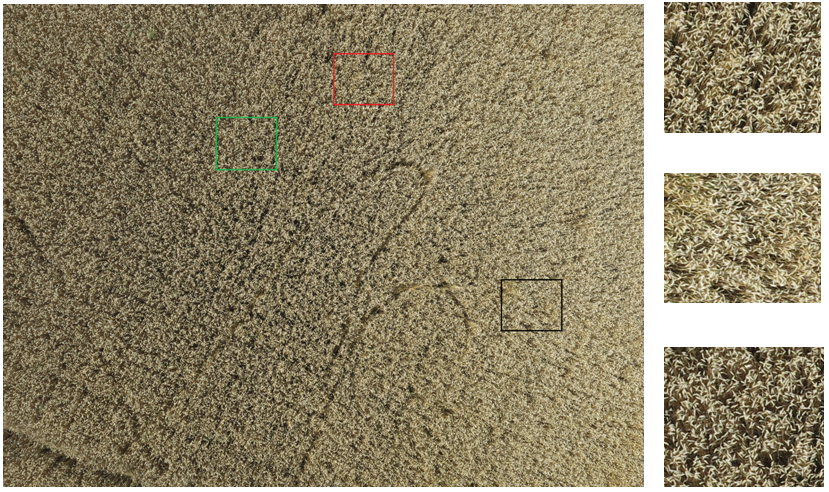
\includegraphics[width=0.65\textwidth]{fig/20.png}
     \vspace{-1em}
    \begin{center}    
       \caption{\textcolor{gray}{\footnotesize \textit{Markbillederne forstørret ind på enkelte korn.}}}
    \label{fig:korn}
     \end{center}
     \vspace{-2.5em}
  \end{figure} \noindent
Disse korn kunne muligvis godt bruges som interessepunkter pga. det store intensitetsskift i området omkring kornet. Problemet er at områderne ligner hinanden så meget, at det måske vil resultere i forkerte korrespondancer. Et andet problem ved kornene er at visse strukturer, der bliver ledt efter, f.eks. hjørner, kan være svært lokaliserbare pga. kornets tilfældige naturlige struktur. \\ \\
Dronens overflyvning af markerne foregår ved at dronen får fire punkter, der definere markens placering. Dronen starter derefter i et hjørne og flyver systematisk fra side til side for at overflyve hele marken. Dronen flyver med én orientation, dvs. der burde ikke være stor grad af rotation imellem billederne. Der forekommer ikke pludselige skift i højden imellem billeder, men derimod en glidende ændring i dronens højde. Generelt er dronens fotografering meget stabil, der forekommer dog visse uregelmæssigheder ved overflyvning som:
\begin{itemize}
\item{\textbf{Overlap:} Billederne overlapper i høj grad hinanden, når dronen befinder sig højt oppe. Dette forøger sandsynligheden for at opnå en repeterbar detektion, da en stor del af punkterne vil indgå i begge billeder. Jo lavere højde dronen befinder sig i, jo mindre overlap forekommer der. Dette sker da dronen bevæger sig i samme hastighed i begge højder, men fanger et større perspektiv på største højde. Detektoren skal derfor indstilles til at kunne finde tilstrækkelig nok punkter, der også gør detektionen mulig på lavere højder. Figur \ref{fig:overlap} viser fire billeder taget ved forskellige højder, sat sammen parvist. Billedernes overlap er markeret med blåt. Billedet (a) er taget, hvor dronen er på største højde, billederne er estimeret til at overlappe med ca. 80 $\%$. Billederne i (b) er taget ved en lavere højde, billederne overlapper hinanden med ca. 35 $\%$. Der kan altså forekomme store ændringer af overlap imellem billederne.
\begin{figure}[H]
    \centering
    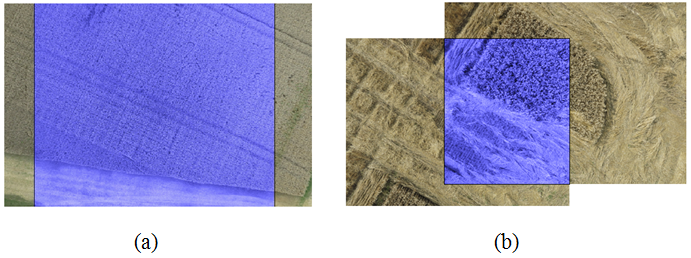
\includegraphics[width=0.65\textwidth]{fig/17.png}
     \vspace{-1em}
    \begin{center}    
       \caption{\textcolor{gray}{\footnotesize \textit{To markbilleder taget fra forskellige højde, det blå område indikere, hvor de to billeder overlapper. (a) Taget ved største højde. (b) Taget ved lavere højde}}}
    \label{fig:overlap}
     \end{center}
     \vspace{-2.5em}
  \end{figure} \noindent }
\item{\textbf{Rotation:} Dronen flyver med samme orientering, den rotere dog lidt når den er nået kanten af marken og skal dreje. Drejningen er vist i figur \ref{fig:rotation}. Denne rotation er ca. mellem 10-15$^{\circ}$. Der forekommer også mindre uregelmæssige rotationer i overflyvningen på mindre end 5$^{\circ}$, højst sandsynligt pga. vind.
\begin{figure}[H]
    \centering
    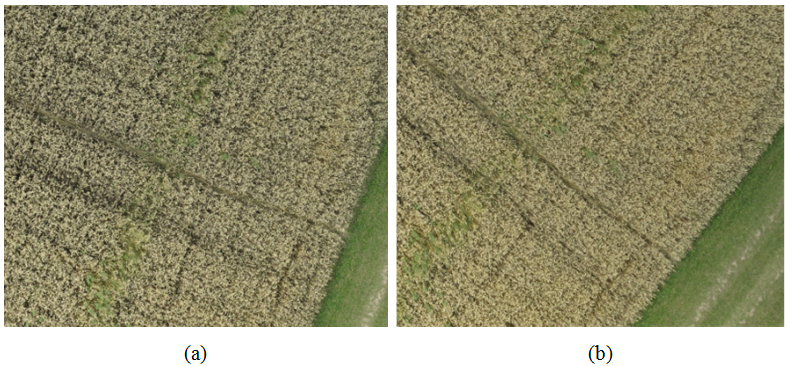
\includegraphics[width=0.65\textwidth]{fig/19.png}
     \vspace{-1em}
    \begin{center}    
       \caption{\textcolor{gray}{\footnotesize \textit{ I billederne er dronen nået til kanten af marken og skal til at ændre retning, hvilket giver rotation i billederne.}}}
    \label{fig:rotation}
     \end{center}
     \vspace{-2.5em}
  \end{figure} \noindent
}
\item{\textbf{Skala:} Korn i markerne forekommer alle på samme skala ift. kameraet, da markerne er flade. I et billede optræder alle objekter derved på samme skala. Der sker dog en ændring af højden som dronen flyver i. Et problem kan opstå, hvis billeder der skal sammenlignes, ikke er taget lige efter hinanden. Det kunne være, hvis dronen flyver henover en mark i y-aksen langsomt faldene og vender tilbage. Skal billederne matches på tværs af x-aksen vil der opstå en større højdeforskel}
\item{\textbf{Vind:} <find eksempler på korn, der skifter retning pga. vind> }
\item{\textbf{Okklusion:}
Okklusion er et problem indenfor computer vision, der omhandler objekter der opstår/forsvinder når kameravinklen forskydes. Okkluderede objekter i et billede kan skabe interesseområder, som ikke optræder i begge billeder. Dette kan også opstå i markbilleder. Når dronen flyver over en mark vil strå, der stikker direkte op imod kameraet placeret på dronen, ses som jord, eller mørke områder pga. jorden. Dvs. i et cirkulært område direkte under dronen vil der opstå et mørkere område. Når dronen flyver videre vil det samme område nu bestå af korn, hvor jorden ikke kan ses, da dronen ikke længere kigger direkte ned i dette område. Dette kan have en stor indflydelse på detektionen, da mørke pletter f.eks. kan opfattes som blobs som kun optræder når dronen befinder sig direkte over området. 
\begin{figure}[H]
    \centering
    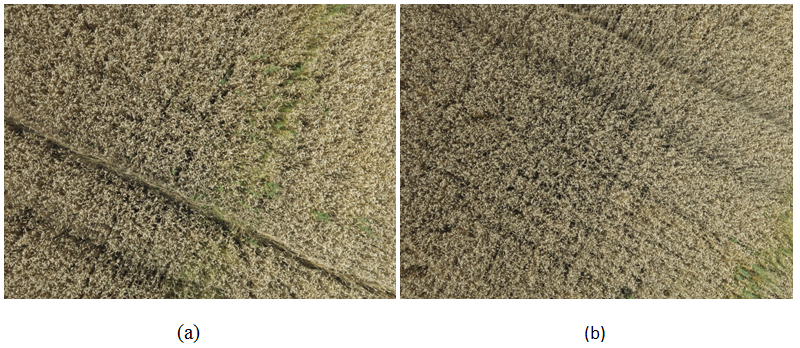
\includegraphics[width=0.65\textwidth]{fig/18.png}
     \vspace{-1em}
    \begin{center}    
       \caption{\textcolor{gray}{\footnotesize \textit{ }}}
    \label{fig:okklusion}
     \end{center}
     \vspace{-2.5em}
  \end{figure} \noindent
Figur \ref{fig:okklusion} er et eksempel på okklusion af korn, hvor traktor spor optræder direkte under dronen og forskudt. Traktorsporet direkte under dronen er meget veldefineret, hvor det forskudte er delvist okkludreret. Det er også værd at bemærke kornet, direkte under dronen, der afgiver mørke pletter. Denne okklusion forekommer umiddelbart kun når dronen er relativt tæt på jorden.}
\end{itemize}
\section{Hypoteser}
Udefra ovenstående analyse kan der opstilles følgende hypoteser til hvad der kræves af de udvalgte metoder:
\begin{itemize}
\item{ Det forventes, grundet strukturen af korn, at detektorer som leder efter veldefineret strukturer, som f.eks. hjørner, ikke vil have en god effekt på korn, men at blobs vil give bedre resultater.}
\item{ Det forventes ikke at metoderne behøver være rotationsinvariante, grundet den lille rotation der forekommer i billederne. }
\item{ Det forventes at metoderne skal være skalainvariante, både pga. den skiftende fotograferingshøjde, men også for at tilpasse detektoren til størrelsen som interessepunkterne forekommer på.}
\item{ Det forventes at der kræves en mange-dimensional\footnote{En deskripor, der indeholder mange informationer} deskriptor, der kan differentiere de forskellige interessepunkter i korn-områder.}
\item{ Det forventes ikke at der kræves affin invarians, da dronen ikke vipper. }
\end{itemize}
Ovenstående hypoteser danner grundlag for udvælgelsen af de korrespondanceanalystiske metoder. Afkræftes hypoteserne vil metoderne forsøges at modificeres/udskiftes ift. disse.